\documentclass{academics}

\academicsCourse{Java 与 Web 开发}{Java and Web Development}
\academicsReport{实验六}{2026 年 5 月 25 日}
\academicsArthur{华博文}{19240212}

\begin{document}

\makeacademicscover

\section{实验环境}

\subsection{操作系统}

macOS 26.4 arm64，Darwin 25.4.0，Apple M5。

\subsection{编程工具}

Visual Studio Code 1.117.0，NeoVim v0.12.0，openjdk 21.0.10。

\subsection{其他工具}

\LaTeX{}，\mil{mjr.py}。

\section{实验内容}

\subsection{第 1 题}

\paragraph{题目描述} {
    编写两个类分别演示两种创建线程的方式：
    \begin{itemize}
        \item 方式一：继承 \mil{Thread} 类，重写 \mil{run()} 方法。
        \item 方式二：实现 \mil{Runnable} 接口，实现 \mil{run()} 方法。
    \end{itemize}
    每个线程执行一个简单的任务：循环打印 $5$ 次当前线程的名称和计数。在 \mil{main} 方法中启动这两个线程，观察输出结果。要求：
    \begin{itemize}
        \item 线程名自定义，例如``继承线程''和``实现线程''。
        \item 使用 \mil{Thread.currentThread().getName()} 获取线程名。
        \item 确保两个线程交替执行（不要求严格交替，但应看到并发效果）。
    \end{itemize}
}

\paragraph{程序实现} {
    \inputminted[label=ExtendThread.java]{java}{../src/P01/ExtendThread.java}
    \inputminted[label=ImplementRunnable.java]{java}{../src/P01/ImplementRunnable.java}
    \inputminted[label=ThreadCreation.java]{java}{../src/P01/ThreadCreation.java}
}

\paragraph{运行结果} {
    \inputminted{text}{../res/P01.out}
}

\subsection{第 2 题}

\paragraph{题目描述} {
    创建一个银行账户类 \mil{Account}，包含私有属性 \mil{balance}（余额）和 \mil{accountNo}（账号）。提供 \mil{withdraw(double amount)} 方法用于取款。要求：
    \begin{itemize}
        \item 当取款金额大于余额时，输出``余额不足''并拒绝操作；否则扣除相应金额，并输出取款成功及当前余额。
        \item 模拟两个线程同时从同一个账户取款：一个线程取款 $800$ 元，另一个线程取款 $1000$ 元，账户初始余额为 $1000$ 元。
        \item 必须使用 \mil{synchronized} 关键字确保线程安全，避免出现余额透支（即两个线程同时取款导致余额变为负数）。
    \end{itemize}
    运行多次，观察是否出现负余额，验证同步正确性。
}

\paragraph{程序实现} {
    \inputminted[label=Account.java]{java}{../src/P02/Account.java}
    \inputminted[label=AccountTest.java]{java}{../src/P02/AccountTest.java}
}

\paragraph{运行结果} {
    \inputminted{text}{../res/P02.out}
}

\subsection{第 3 题}

\paragraph{题目描述} {
    使用 \mil{wait()} 和 \mil{notify()} 实现经典的生产者-消费者模型：
    \begin{itemize}
        \item 创建一个共享缓冲区 \mil{Buffer}，容量为 $1$（只能存放一个整数）。
        \item 生产者线程产生 $1$ 到 $10$ 的整数，放入缓冲区，每放入一个后等待消费者取走。
        \item 消费者线程从缓冲区取出整数并打印，每取走一个后通知生产者继续生产。
        \item 要求生产者和消费者交替执行，顺序输出``生产$x$''和``消费$x$''。
    \end{itemize}
    使用 \mil{synchronized} 块控制对缓冲区的访问，在缓冲区满时生产者等待，缓冲区空时消费者等待。
}

\paragraph{程序实现} {
    \inputminted[label=Buffer.java]{java}{../src/P03/Buffer.java}
    \inputminted[label=ProducerConsumer.java]{java}{../src/P03/ProducerConsumer.java}
}

\paragraph{运行结果} {
    \inputminted{text}{../res/P03.out}
}

\subsection{第 4 题}

\paragraph{题目描述} {
    模拟一个场景：主线程需要等待多个子线程全部完成某项准备工作后，才能继续执行。使用 \mil{CountDownLatch} 实现：
    \begin{itemize}
        \item 创建 $3$ 个子线程，每个子线程随机休眠一段时间（模拟准备工作），然后打印``XX准备就绪''，并调用 \mil{countDown()}。
        \item 主线程调用 \mil{await()} 等待，直到所有子线程准备就绪后，输出``所有准备工作完成，主线程开始执行''。
    \end{itemize}
    验证主线程确实在所有子线程完成之后才继续。
}

\paragraph{程序实现} {
    \inputminted[label=CountDownLatchDemo.java]{java}{../src/P04/CountDownLatchDemo.java}
}

\paragraph{运行结果} {
    \inputminted{text}{../res/P04.out}
}

\subsection{第 5 题}

\paragraph{题目描述} {
    不使用 \mil{synchronized}，而是使用 \mil{AtomicInteger} 实现一个线程安全的计数器。要求：
    \begin{itemize}
        \item 创建一个计数器类 \mil{Counter}，包含一个 \mil{AtomicInteger} 类型的私有变量。
        \item 提供 \mil{increment()} 方法使计数器加 $1$，\mil{getValue()} 方法返回当前值。
        \item 创建 $10$ 个线程，每个线程对计数器执行 $1000$ 次 \mil{increment()} 操作。
        \item 主线程等待所有线程结束后，输出计数器的最终值，验证是否为 $10 \times 1000 = 10000$。
        \item 如果不使用原子类，用普通 \mil{int} 会出现数据竞争导致结果小于 $10000$，此处验证原子类的正确性。
    \end{itemize}
    多次运行程序，结果始终为 $10000$，证明原子性。
}

\paragraph{程序实现} {
    \inputminted[label=Counter.java]{java}{../src/P05/Counter.java}
    \inputminted[label=AtomicCounter.java]{java}{../src/P05/AtomicCounter.java}
}

\paragraph{运行结果} {
    \inputminted{text}{../res/P05.out}
}

\subsection{第 6 题}

\paragraph{题目描述} {
    设计一个 Java 程序，完成：二叉树的存储与读取。
    程序在内存中构成一棵二叉树，如下图所示。将该二叉树通过对象序列化的方式，直接保存到文件 \mil{tree.ser} 中。然后再从该 \mil{tree.ser} 文件中读取该树，在内存中重新构造出该树。
    \begin{figure}[h]
        \centering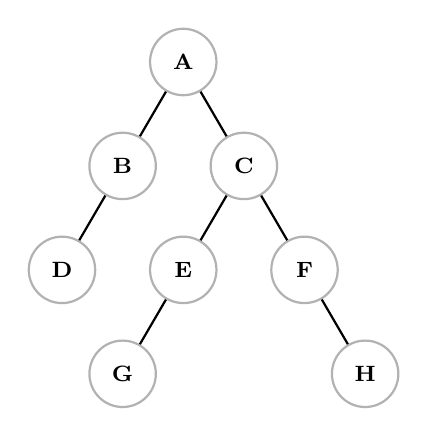
\begin{tikzpicture}[
    tnode/.style={
        circle, thick, draw=gray!60, fill=white,
        minimum size=24pt, inner sep=0pt,
        font=\bfseries\footnotesize
    },
    ledge/.style={thick},
    redge/.style={thick},
    scale=1.1,
]

% dx = 0.7, dy = 1.2
\node [tnode] (A) at (0.0, 0.0) {A};
\node [tnode] (B) at (-0.7,-1.2) {B};
\node [tnode] (C) at ( 0.7,-1.2) {C};
\node [tnode] (D) at (-1.4,-2.4) {D};
\node [tnode] (E) at ( 0.0,-2.4) {E};
\node [tnode] (F) at ( 1.4,-2.4) {F};
\node [tnode] (G) at (-0.7,-3.6) {G};
\node [tnode] (H) at ( 2.1,-3.6) {H};

\draw[ledge] (A) -- (B);
\draw[redge] (A) -- (C);
\draw[ledge] (B) -- (D);
\draw[ledge] (C) -- (E);
\draw[redge] (C) -- (F);
\draw[ledge] (E) -- (G);
\draw[redge] (F) -- (H);

\end{tikzpicture}

    \end{figure}
}

\paragraph{程序实现} {
    \inputminted[label=TreeNode.java]{java}{../src/P06/TreeNode.java}
    \inputminted[label=BinaryTreeSerialize.java]{java}{../src/P06/BinaryTreeSerialize.java}
}

\paragraph{运行结果} {
    \inputminted{text}{../res/P06.out}
}

\end{document}
